\documentclass[a4paper]{article}
\usepackage[italian]{babel}
\usepackage[T1]{fontenc}
\usepackage[utf8]{inputenc}
\usepackage{soulutf8}
\usepackage{graphicx}
\usepackage{imakeidx}
\usepackage{enumitem}
\usepackage{amsfonts}
\usepackage{titlesec}
\usepackage{xcolor}
\definecolor{newcolor}{HTML}{e6e6e6} %9fdfbf - c6ecd9
\usepackage{soul} %for \hl
\sethlcolor{newcolor}
\newcommand{\sectionbreak}{\clearpage}
\makeindex[intoc]
\usepackage[hyperfootnotes=false, colorlinks=true, linkcolor=black, urlcolor=black]{hyperref}

\begin{document}
\title{Basi di Dati in Pillole}
\author{\href{https://t.me/amarusofia}{Sofia Amarù}}
\maketitle
\tableofcontents

\section*{Note}
Il seguente testo è un personalissimo specchietto riassuntivo dei concetti fondamentali studiati durante il corso di Basi di Dati (corso di laurea triennale in Informatica presso l'Università degli Studi di Milano-Bicocca) e lo studio sullo stesso non è sufficiente per il superamento dell'esame. Si consiglia la lettura solo dopo aver studiato dal libro \emph{Basi di Dati - Modelli e linguaggi di interrogazione} degli autori Azteni, Ceri, Paraboschi, Torlone.\medskip\\
Questo testo può contenere errori: nell'eventualità vi prego di contattarmi per procedere alla correzione.\medskip\\
%
Ricordo ai miei compagni che l'esame è composto da 5 esericizi relativi ai seguenti argomenti:
\begin{itemize}[leftmargin=*, noitemsep]
  \item Modello ER
  \item Modello Relazionale
  \item Progettazione logica
  \item SQL
  \item Algebra relazionale
\end{itemize}

\section{Introduzione}
\subsection{Concetti fondamentali}
\subsubsection{Sistema informativo, sistema informatico, dati}

\hl{sistema informativo}: componente (non necessariamente automatizzata) di un’organizzazione, che gestisce le informazioni di interesse\medskip\\
%
\hl{sistema informatico}: porzione automatizzata del sistema informativo
\begin{itemize}[noitemsep]
  \item acquisizione e memorizzazione
  \item aggiornamento
  \item interrogazione
  \item elaborazione
\end{itemize}
%
\hl{dato $\neq$ informazione}
\begin{itemize}[noitemsep]
  \item dato: non ha alcun valore fino a quando non viene interpretato (immutato nel tempo)
  \item informazione: si ha quando un dato viene interpretato
\end{itemize}

\subsubsection{Definizione di database, DBMS}
\hl{DATABASE}: collezione di dati usati per rappresentare informazioni di interesse\\
\hl{DBMS (data base managment system)}: software per la gestione di DB

\subsubsection{Caratteristiche}
caratteristiche di un DB:
\begin{itemize}[noitemsep]
  \item privatezza
  \item affidabilità
  \item efficienza
  \item efficacia
\end{itemize}
%
fasi:
\begin{itemize}[noitemsep]
  \item definizione
  \item creazione e popolazione
  \item manipolazione
\end{itemize}
%
caratteristiche di un sistema di DB:
\begin{itemize}[noitemsep]
  \item natura autodescrittiva
  \item separazione tra programmi e dati
  \item astrazione dei dati (visione concettuale del DB per l'utente)
  \item supporto viste multiple dei dati
  \item condivisione dei dati e gestione con utenti multipli
\end{itemize}
%
\subsubsection{Modelli}
\hl{modello logico:}
\begin{itemize}[noitemsep]
  \item \hl{relazionale} (costruttore relazione; record a struttura fissa; tabella)
  \item gerarchico (strutture ad albero)
  \item reticolare (grafi)
  \item a oggetti
  \item XML
\end{itemize}
\hl{modello concettuale:}
\begin{itemize}[noitemsep]
  \item \hl{ER} (entità-relazione)
\end{itemize}

\subsubsection{Transizioni, schema, istanza}
transizione: insieme indivisibile di operazioni\medskip\\
%
\hl{schema}: struttura, invariante nel tempo\\
\hl{istanza}: valori attuali, possono cambiare anche molto rapidamente

\subsubsection{Livelli di astrazione}
\hl{schema logico} - descrizione dell’intera base di dati per mezzo del modello logico\\
\hl{schema interno} - rappresentazione dello schema logico per mezzo di strutture fisiche di memorizzazione\\
\hl{schema esterno} - descrizione di una porzione della base di dati per mezzo del modello logico. A volte non è esplicitamente presente ma è possibile definire relazioni derivate (viste)

\subsubsection{Indipendenza dei dati}
\hl{indipendenza fisica} - interagire col DBMS indipendentemente dalla struttura fisica dei dati\\
\hl{indipendenza logica} - interagire col livello esterno indipendentemente dal livello logico

\subsubsection{Linguaggi}
\hl{DDL Data Definition Language} - definizione degli schemi e delle autorizzazioni per l’accesso\\
\hl{DML Data Manipulation Language} - interrogazione e aggiornamento delle istanze del DB

\section{Modello ER (entità-relazione)}
\subsection{Rappresentazione grafica dei costrutti}
\begin{center}
      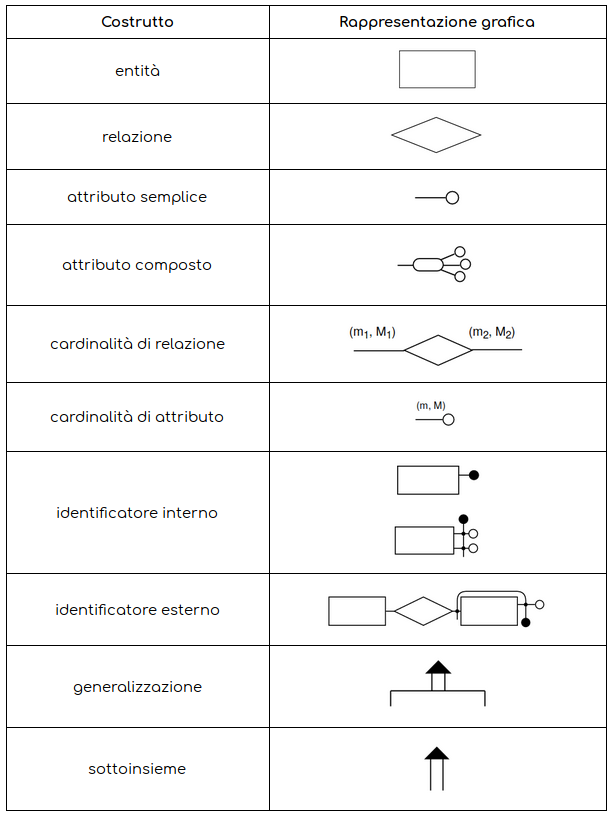
\includegraphics[scale=0.6]{img/er1.png}
\end{center}

\subsection{Costrutti}
\hl{entità} - classe di oggetti con proprietà comuni (il nome va al singolare)\medskip\\
\hl{relazione} - legame logico (il nome deve essere univoco; è preferibile usare un sostantivo per evitare di assegnare un verso)\medskip\\
\hl{attributo composto} - raggruppamento di attributi (Es. Via, Numero, CAP)\medskip\\
\hl{cardinalità} di relazione - indica quante volte, in una relazione, l'occorrenza dell'entità è legata ad occorrenze dell'altra entità
\begin{center}
      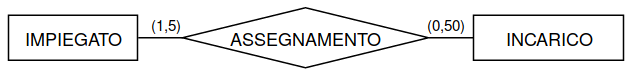
\includegraphics[scale=0.5]{img/er4.png}\\
      un impiegato ha da 1 a 5 incarichi
    \end{center}
\hl{identificatore (chiave)} - identificatore univoco dell’entità\medskip\\
\hl{identificatore interno} - se è uno o più attributi di un’entità
\begin{center}
      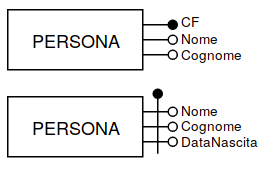
\includegraphics[scale=0.5]{img/er2.png}
\end{center}
\hl{identificatore esterno} - se un’entità viene identificata da un attributo di un’altra entità con cui ha una relazione
\begin{center}
      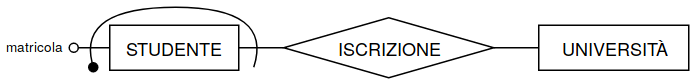
\includegraphics[scale=0.5]{img/er3.png}
\end{center}
\hl{generalizzazione totale} - non esistono altri figli
\begin{center}
      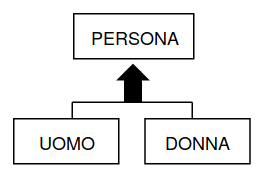
\includegraphics[scale=0.5]{img/er5.png}
\end{center}
\hl{generalizzazione parziale} - ci possono essere altri figli
\begin{center}
      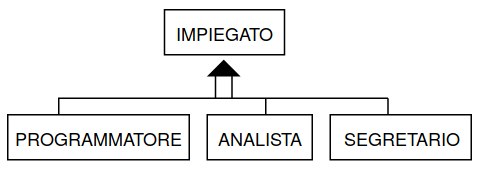
\includegraphics[scale=0.5]{img/er6.png}
\end{center}
\hl{sottoinsieme} - unsolo figlio\medskip\\
\hl{generalizzazione esclusiva} - es. uomo-donna (o è uomo o è donna)\medskip\\
\hl{generalizzazione sovrapposta} - es. studente-lavoratore (può essere studente, lavoratore o studente-lavoratore)

\section{Modello Relazionale}
\subsection{Vincoli di integrità}
\hl{intrarelazionale} - soddisfatto rispetto a singole relazioni
\begin{itemize}
  \item[] \hl{di tupla} -  può essere valutato su ciascuna tupla indipendentemente dalle altre.\\
  Es. la lode può comparire solo con voto 30
  \item[] \hl{di dominio} - restrizione sul dominio dell’attributo\\
  Es. voto compreso tra 18 e 30
\end{itemize}
\hl{interrelazionale} - coinvolge più relazioni
\begin{itemize}
  \item[] \hl{vincolo di integrità referenziale} - proprietà dei dati che per essere soddisfatta richiede che ogni valore di un attributo (colonna) di una relazione (tabella) esista come valore di un altro attributo in un'altra relazione.\\
  Es. matricola compare in ESAMI solo se compare in STUDENTI
\end{itemize}

\subsection{Chiave, superchiave, superchiave minimale}
\hl{chiave} - insieme di attributi utilizzato per identificare univocamente le tuple di una relazione\medskip\\
\hl{superchiave} - insieme di attributi di una relazione tali che le relative tuple sono tutte diverse tra loro (identificazione univoca)\medskip\\
\hl{superchiave minimale} - superchiave che non contiene una superchiave\medskip\\
\hl{chiave primaria} - chiave a cui non è permesso contenere valori nulli (la presenza di NULL impedisce l’identificazione univoca)

\section{Progettazione logica}
\subsection*{Fasi}
\begin{itemize}[noitemsep, leftmargin=*]
  \item \hl{Ristrutturazione schema ER}
        \begin{itemize}[noitemsep]
          \item Analisi delle ridondanze
          \item Eliminazione delle generalizzazioni
          \item Partizionamento/accorpamento entità e associazioni
          \item Scelta identificatori principali
        \end{itemize}
  \item \hl{Traduzione verso modello logico}
\end{itemize}

\subsection{Ristrutturazione schema ER}
\subsubsection{Analisi delle ridondanze}
La presenza di un dato ridondante comporta:
\begin{itemize}[noitemsep]
  \item[$\times$] occupazione memeoria
  \item[$\times$] operazioni per mantenere dato aggiornato
  \item[\checkmark] riduzione accessi necessari per calcolarlo
\end{itemize}

\subsubsection{Eliminazione delle generalizzazioni}
\hl{Accorpamento dei figli nel genitore}
\begin{center}
      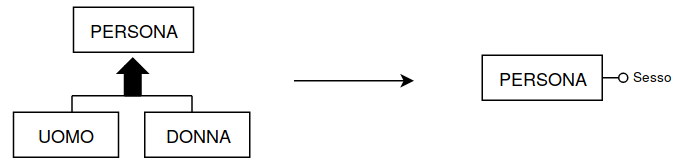
\includegraphics[scale=0.45]{img/pl1.png}
\end{center}
%
\hl{Accorpamento del genitore dei figli}\\
NB. Possibile solo se la generalizzazione è totale!
\begin{center}
      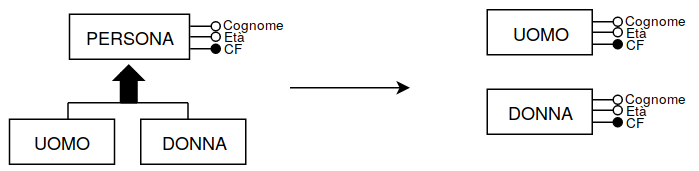
\includegraphics[scale=0.45]{img/pl2.png}
\end{center}
%
\hl{Sosituzione generalizzazioni con associazioni}\\
NB. Conveniente con generalizzazione parziale
\begin{center}
      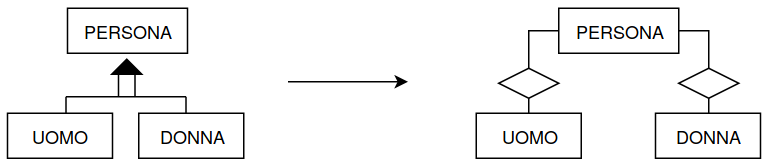
\includegraphics[scale=0.45]{img/pl3.png}
\end{center}

\subsubsection{Partizionamento}
\hl{decomposizione verticale}
\begin{center}
      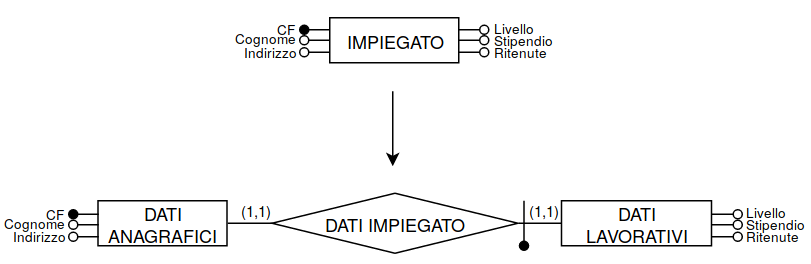
\includegraphics[scale=0.45]{img/pl4.png}
\end{center}
%
\hl{decomposizione orizzontale}
\begin{center}
      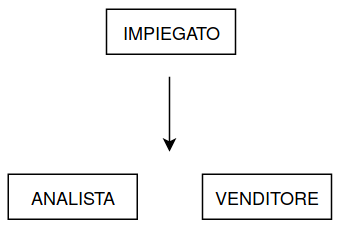
\includegraphics[scale=0.45]{img/pl5.png}
\end{center}

\subsubsection{Eliminazione di attributi multivalore}
Es. Un'agenzia può avere più numeri di telefono
\begin{center}
      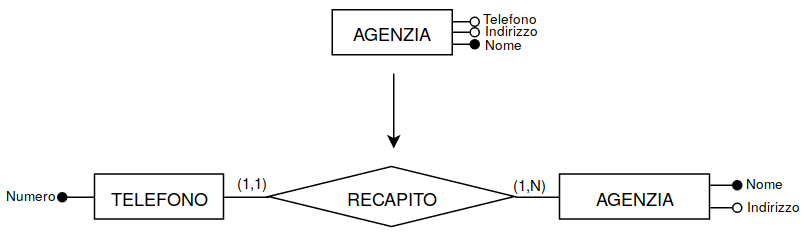
\includegraphics[scale=0.44]{img/pl6.png}
\end{center}

\subsubsection{Accorpamento di entità}
NB. Solitamente su associazioni uno a uno
\begin{center}
      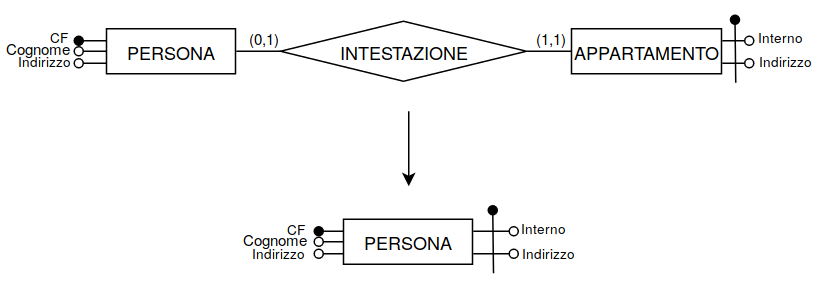
\includegraphics[scale=0.44]{img/pl7.png}
\end{center}

\subsubsection{Scelta degli identificatori principali}
\begin{itemize}[noitemsep]
  \item No attributi con valori nulli
  \item Preferire identificatore composto da 1 o \textbf{pochi} attributi
  \item Preferire identificatore interno ad intentificatore esterno
  \item Preferire identificatore che viene utilizzato da molte operazioni per accedere alle occorrenze dell'entità
\end{itemize}

\subsection{Traduzione verso modello logico}
\subsubsection{Molti a molti}
\begin{center}
      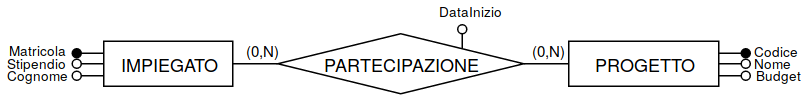
\includegraphics[scale=0.44]{img/pl8.png}
\end{center}
%
IMPIEGATO(\underline{Matricola}, Cognome, Stipendio)\\
PROGETTO(\underline{Codice}, Nome, Budget)\\
PARTECIPAZIONE(\underline{Impiegato}, \underline{Progetto}, DataInizio)\medskip\\
%
\hl{NB.} \underline{Impiegato} è la ridenominazione di \underline{Matricola} e \underline{Progetto} è la ridenominazione di \underline{Codice}

\subsubsection{Uno a molti}
\begin{center}
      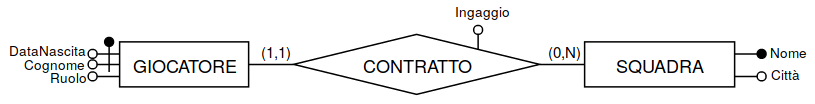
\includegraphics[scale=0.44]{img/pl9.png}
\end{center}
%
GIOCATORE(\underline{DataNascita}, \underline{Cognome}, Ruolo)\\
SQUADRA(\underline{Nome}, Città)\\
CONTRATTO(\underline{Giocatore}, Squadra, Ingaggio)\medskip\\
%
diventa\medskip\\
%
GIOCATORE(\underline{DataNascita}, \underline{Cognome}, Ruolo, Squadra, Ingaggio)\\
SQUADRA(\underline{Nome}, Città)

\subsubsection{Uno a uno con partecipazioni obbligatorie per entrambe le entità}
\begin{center}
      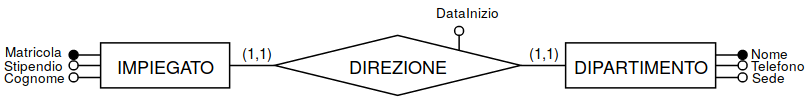
\includegraphics[scale=0.44]{img/pl10.png}
\end{center}
%
DIRETTORE(\underline{Matricola}, Cognome, Stipendio, Dipartimento, InizioDirezione)\\
DIPARTIMENTO(\underline{Nome}, Telefono, Sede)\medskip\\
%
oppure\medskip\\
%
DIRETTORE(\underline{Matricola}, Cognome, Stipendio)\\
DIPARTIMENTO(\underline{Nome}, Telefono, Sede, Direttore, InizioDirezione)

\subsubsection{Uno a uno con partecipazione opzionale per una sola entità}
\begin{center}
      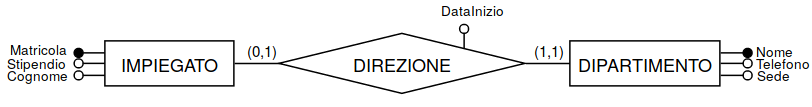
\includegraphics[scale=0.44]{img/pl11.png}
\end{center}
%
IMPIEGATO(\underline{Matricola}, Cognome, Stipendio)\\
DIPARTIMENTO(\underline{Nome}, Telefono, Sede)\\
DIREZIONE(\underline{Direttore}, Dipartimento, DataInizio)

\section{SQL}
\hl{Structured Query Language}, contiene funzionalità di un \hl{DDL} (Data Definition Language) e di un \hl{DML} (Data Manipulation Language)\medskip\\

\subsection{Interrogazioni}
\begin{center}
      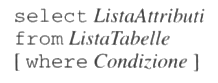
\includegraphics[scale=0.5]{img/sql1.png}\\
      esempio di interrogazione
\end{center}

\subsection{Select, from, where}
clausola \hl{\texttt{select}} (target list) - specifica gli elementi dello schema della tabella risultato. Come argomento può comparire * , che rappresenta tutti gli attributi delle tabelle elencate nella clausola from.\medskip\\
%
clausola \hl{\texttt{from}} - ha come argomento l’insieme delle tabelle a cui si vuole accedere. Sul prodotto cartesiano delle tabelle vengono applicate le condizioni contenute nella clausola where.\medskip\\
%
clausola \hl{\texttt{where}} - ha come argomento un’espressione booleana\medskip\medskip\medskip\\
%
Consideriamo le due tabelle\\
IMPIEGATO(\underline{Nome}, \underline{Cognome}, Dipart, Ufficio, Stipendio, CIttà)\\
DIPARTIMENTO(\underline{Nome}, Indirizzo, Città)
\begin{enumerate}[leftmargin=*]
  \item estrarre lo stipendio degli impiegati di nome “Rossi”.
  \begin{verbatim}
  select Stipendio as Salario
  from Impiegato
  where Cognome = ‘Rossi’
  \end{verbatim}

  \item estrarre tutte le informazioni relative agli impiegati di cognome “Rossi”
  \begin{verbatim}
  select *
  from Impiegato
  where Cognome = ‘Rossi’
  \end{verbatim}

  \item estrarre lo stipendio mensile dell’impiegato che ha cognome “Bianchi”
  \begin{verbatim}
  select Stipendio/12 as StipendioMensile
  from Impiegato
  where Cognome = ‘Bianchi’
  \end{verbatim}

  \item estrarre i nomi degli impiegati e le città in cui lavorano
  \begin{verbatim}
  select Impiegato.Nome, Impiegato.Cognome, Dipartimento.Città
  from Impiegato, Dipartimento
  where Impiegato.Dipart = Dipartimento.Nome
  \end{verbatim}

  \item gli attributi per cui sorge un'ambiguità sono Nome e Città. L'interrogazione precedente può essere espressa facendo uso degli alias per le tabelle allo scopo di abbreviare i riferimenti a esse.
  \begin{verbatim}
  select I.Nome, Cognome, D.Città
  from Impiegato as I, Dipartimento as D
  where Dipart = D.Nome
  \end{verbatim}

  \item estrarre nome e cognome degli impiegato che lavorano nell’ufficio 20 del dipartimento Amministrazione.
  \begin{verbatim}
  select Nome, Cognome
  from Impiegato
  where Ufficio = 20 and Dipart = ‘Amministrazione’
  \end{verbatim}

  \item estrarre i nomi e i cognomi degli impiegati che lavorano nel dipartimento Amministrazione o nel dipartimento Produzione
  \begin{verbatim}
  select Nome, Cognome
  from Impiegato
  where Dipart = ‘Amministrazione’ or
        Dipart = ‘Produzione’
  \end{verbatim}

  \item estrarre i nomi propri degli impiegati di nome “Rossi” che lavorano nei dipartimenti Amministrazione o Produzione
  \begin{verbatim}
  select Nome
  from Impiegato
  where Cognome = ‘Rossi’ and
        (Dipart = ‘Amministrazione’ or
        Dipart = ‘Produzione’)
  \end{verbatim}
\end{enumerate}

\subsection{Is null}
predicato \hl{is null} - per selezionare termini con valori nulli ($\neg$ \hl{is not null})

\subsection{Distinct, all}
parola chiave \hl{distinct} - per eliminare i duplicati ($\neg$ \hl{all}, di default, opzionale)\medskip\medskip\medskip\\
%
Consideriamo la relazione\\
PERSONA(\underline{CodFiscale}, Nome, Cognome, Città)
%
\begin{enumerate}[leftmargin=*]
  \setcounter{enumi}{8}
  \item estrarre le città delle persone con cognome “Rossi”, facendo comparire ogni città al più una volta
  \begin{verbatim}
  select distinct Città
  from Persona
  where Cognome = ‘Rossi’
  \end{verbatim}
\end{enumerate}

\subsection{Join, alias}
operatore \hl{join} - si scrive nell’ambito della clausola from, e non compare il where. (inner, right, left, full)
\begin{enumerate}[leftmargin=*]
  \setcounter{enumi}{9}
  \item riscrivi il punto 5.
  \begin{verbatim}
  select I.Nome, Cognome, D.Città
  from Impiegato I join Dipartimento D
       on Dipart = D.Nome
  \end{verbatim}

  \item estrarre tutti gli impiegati che hanno lo stesso cognome (ma diverso nome) di impiegati del dipartimento Produzione
  \begin{verbatim}
  select I1.Nome, I1.Cognome
  from Impiegato I1, Impiegato I2
  where I1.Cognome = I2.Cognome and
        I1.Nome <> I2.Nome and
        I2.Dipart = ‘Produzione’
  \end{verbatim}
  immaginiamo che al momento della definizione degli \hl{alias} (\texttt{I1} e \texttt{I2}) vengano create due diverse tabelle che verranno confrontate tra di loro.
\end{enumerate}

\subsection{Order by}
clausola \hl{order by} - ordina in modo ascendente (\hl{asc}) o discendente (\hl{desc})
\begin{enumerate}[leftmargin=*]
  \setcounter{enumi}{11}
  \item estrarre il contenuto della tabella AUTOMOBILE ordinato in base alla marca (in modo discendente) e al modello
  \begin{verbatim}
  select *
  from Automobile
  order by Marca desc, Modello
  \end{verbatim}
\end{enumerate}

\subsection{Operatori aggregati}
\hl{count} - torna il numero degli attributi\\
\hl{sum} - torna la somma dei valori dell’espressione\\
\hl{max} - massimo\\
\hl{min} - minimo\\
\hl{avg} - media dei valori
\begin{enumerate}[leftmargin=*]
  \setcounter{enumi}{12}
  \item estrarre il numero di diversi valori dell’attributo Stipendio fra tutte le righe di IMPIEGATO
  \begin{verbatim}
  select count (distinct Stipendio)
  from Impiegato
  \end{verbatim}
\end{enumerate}

\subsection{Group by}
clausola \hl{group by} - raggruppa per
\begin{enumerate}[leftmargin=*]
  \setcounter{enumi}{13}
  \item estrarre la somma degli stipendi di tutti gli impiegati dello stesso dipartimento
  \begin{verbatim}
  select Dipart, sum(Stipendio)
  from Impiegato
  group by Dipartimento
  \end{verbatim}
\end{enumerate}

\subsection{Predicati su gruppi: having}
predicato \hl{having} - che ha
\begin{enumerate}[leftmargin=*]
  \setcounter{enumi}{14}
  \item estrarre i dipartimenti che spendono più di 100 mila euro in stipendi
  \begin{verbatim}
  select Dipart, sum(Stipendio) as SommaStipendi
  from Impiegato
  group by Dipart
  having sum(Stipendio) > 100
  \end{verbatim}
\end{enumerate}

\subsection{Interrogazioni di tipo insiemistico}
\hl{union}\\
\hl{intersect}\\
\hl{except}
\begin{enumerate}[leftmargin=*]
  \setcounter{enumi}{15}
  \item estrarre i nomi e i cognomi degli impiegati
  \begin{verbatim}
  select Nome
  from Impiegato
        union
  select Cognome
  from Impiegato
  \end{verbatim}
\end{enumerate}

\subsection{Any}
clausola \hl{any} - la riga soddisfa la condizione se è vero il confronto tra il valore dell’attributo per la riga e almeno uno degli elementi restituiti dall’interrogazione
\begin{enumerate}[leftmargin=*]
  \setcounter{enumi}{16}
  \item estrarre gli impiegati che lavorano in dipartimenti situati a Firenze
  \begin{verbatim}
  select *
  from Impiegato
  where Dipart = any (select Nome
                      from Dipartimento
                      where Città = ‘Firenze’)
  \end{verbatim}
\end{enumerate}


\section{Algebra relazionale}
\hl{Relazione}: insieme di tuple omogenee.

\subsection{Operatori insiemistici}
\hl{unione} $\cup$ \\
\hl{intersezione} $\cap$\\
\hl{differenza} $-$
\begin{center}
      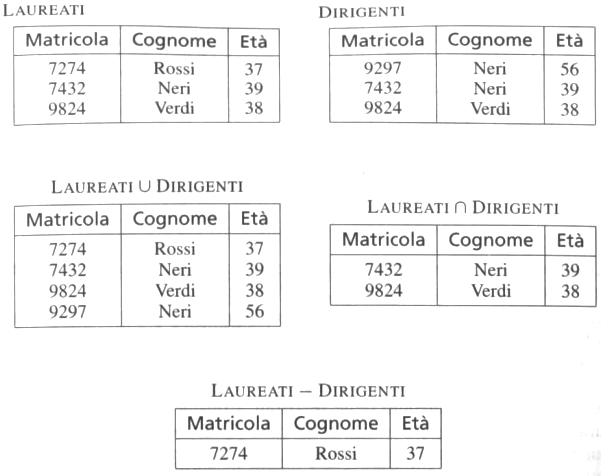
\includegraphics[scale=0.45]{img/ar1.png}
\end{center}

\subsection{Operatori principali}
\subsubsection{Ridenominazione}
Agisce solo sullo schema, cambiando solo i nomi degli attributi
\[\rho_{\textbf{nuovo nome}\leftarrow \textbf{vecchio nome}}\]
\begin{center}
      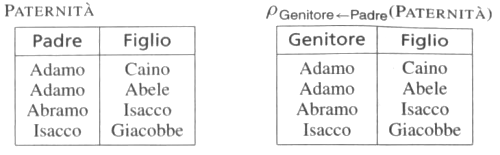
\includegraphics[scale=0.45]{img/ar2.png}
\end{center}

\subsubsection{Selezione}
Produce un sottoinsieme delle tuple su tutti gli attributi (decomposizione orizzontale)
\[\sigma_{\textbf{condizione di selezione}}\]
\begin{center}
      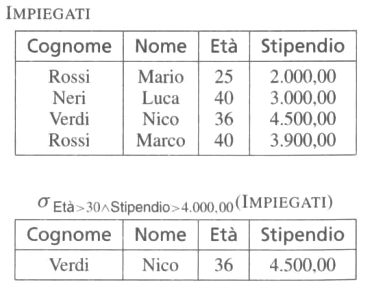
\includegraphics[scale=0.45]{img/ar3.png}
\end{center}

\subsubsection{Proiezione}
È l’insieme delle tuple ottenute considerando solo i valori dei campi scelti. La proiezione contiene lo stesso numero di tuple della relazione di partenza solo se i campi scelti sono una superchiave. (decomposizione verticale)
\[\pi_{\textbf{campi scelti}}\]
\begin{center}
      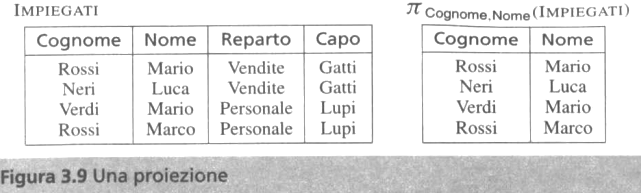
\includegraphics[scale=0.45]{img/ar4.png}\\
      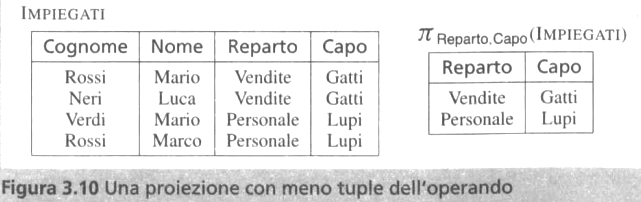
\includegraphics[scale=0.45]{img/ar5.png}
\end{center}

\subsubsection{Join}
Permette di correlare dati contenuti in relazioni diverse
\[\Join\]
%
\hl{join naturale} - correla dati in relazioni diverse sulla base di valori uguali in campi uguali.
\begin{center}
      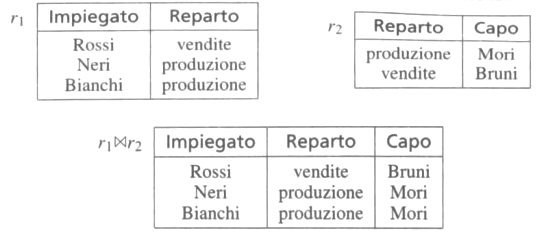
\includegraphics[scale=0.45]{img/ar6.png}
\end{center}
%
\hl{join completo} - ogni tupla contribuisce ad almeno una tupla del risultato (vedi immagine sopra)\medskip\\
%
\hl{join con tuple dangling} - alcune tuple non contribuiscono al risultato
\begin{center}
      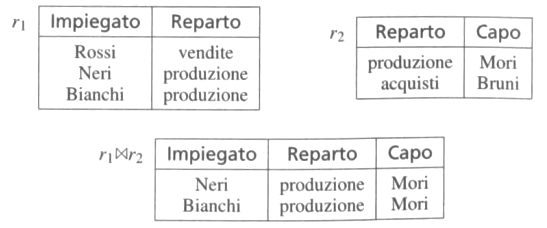
\includegraphics[scale=0.45]{img/ar7.png}
\end{center}
%
\hl{join esterni} - tutte le tuple contribuiscono al risultato, eventualmente estese con valori nulli
\begin{itemize}[noitemsep]
  \item [-] sinistro
  \item [-] destro
  \item [-] completo
\end{itemize}
\begin{center}
      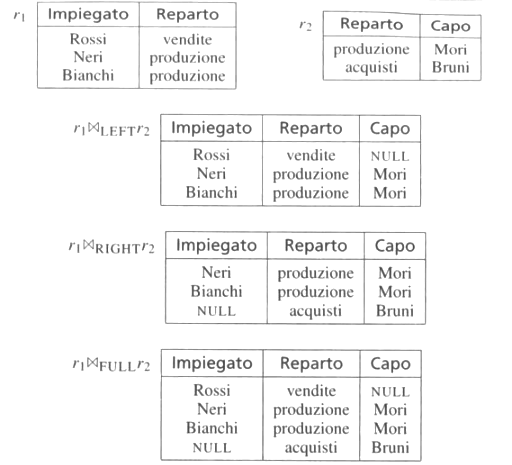
\includegraphics[scale=0.45]{img/ar8.png}
\end{center}

\subsubsection{Prodotto cartesiano}
Il risultato è la combinazione delle tuple in tutti i modi possibili.\\
\hl{NB}. il termine è improprio: il prodotto cartesiano di due insiemi è un insieme di coppie, qui abbiamo tuple.
\begin{center}
      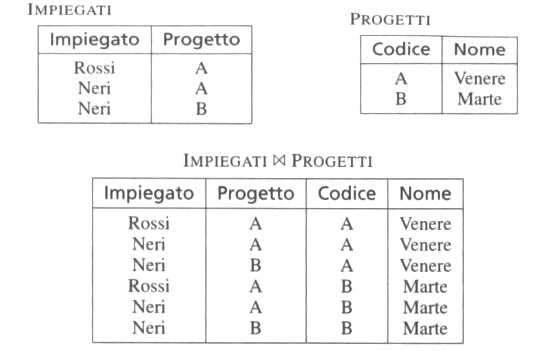
\includegraphics[scale=0.45]{img/ar9.png}
\end{center}

\subsubsection{Theta join e equi-join}
\hl{theta join} - operatore derivato, prodotto cartesiano + selezione\medskip\\
\hl{equi-join} - theta join in cui la condizione di selezione è una congiunzione di atomi di uguaglianza con un attributo della prima relazione
\begin{center}
      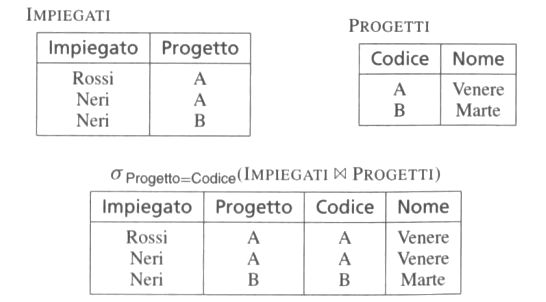
\includegraphics[scale=0.45]{img/ar10.png}
\end{center}

\subsubsection{Logica a tre valori}
vero (V), falso (F), sconosciuto (U)
\begin{center}
      
\includegraphics[scale=0.45]{img/ar11.png}
\end{center}

\subsubsection{Interrogazioni}
\hl{Interrogazione}: funzione che, applicata alla base di dati, produce relazioni.

\end{document}
